% Generated by pipeline/paper/scripts/make_result_figures.py. Do not edit by hand.
% PROJECTED closed form (1-0.01)^n. The curve is the formula, not a fit. The marked point is the savings-job probe size.
% Shared figure style. Input once; a second input is a no-op.
\ifdefined\actsplotsready
\else
  \def\actsplotsready{1}
  \colorlet{actsteal}{teal!72!black}
  \colorlet{actstealfaint}{teal!16}
  \colorlet{actsorange}{orange!88!black}
  \colorlet{actsink}{black!80}
  \colorlet{actsghost}{black!45}
  \colorlet{actsfail}{red!62!black}
  \colorlet{actsrule}{black!50}
  \usetikzlibrary{intersections}
  \usepgfplotslibrary{fillbetween,groupplots}
  \pgfplotsset{
    acts/.style={
      font=\scriptsize\sffamily,
      tick label style={font=\scriptsize\sffamily},
      label style={font=\scriptsize\sffamily},
      legend style={
        font=\scriptsize\sffamily,
        draw=none,
        fill=none,
        cells={anchor=west},
        inner sep=1pt,
        column sep=6pt
      },
      legend cell align=left,
      scale only axis,
      clip=false,
      axis line style={actsrule},
      tick style={actsrule},
      tick align=outside,
      axis lines=left,
      xmajorgrids=true,
      major grid style={black!7},
      ymajorgrids=false,
      every node/.append style={font=\scriptsize\sffamily, inner sep=1.5pt},
      every axis plot/.append style={line join=round, line cap=round},
    },
  }
  \tikzset{
    actlab/.style={
      font=\scriptsize\sffamily,
      fill=white,
      fill opacity=0.92,
      text opacity=1,
      inner sep=1.35pt,
      outer sep=0.5pt,
    },
  }
\fi

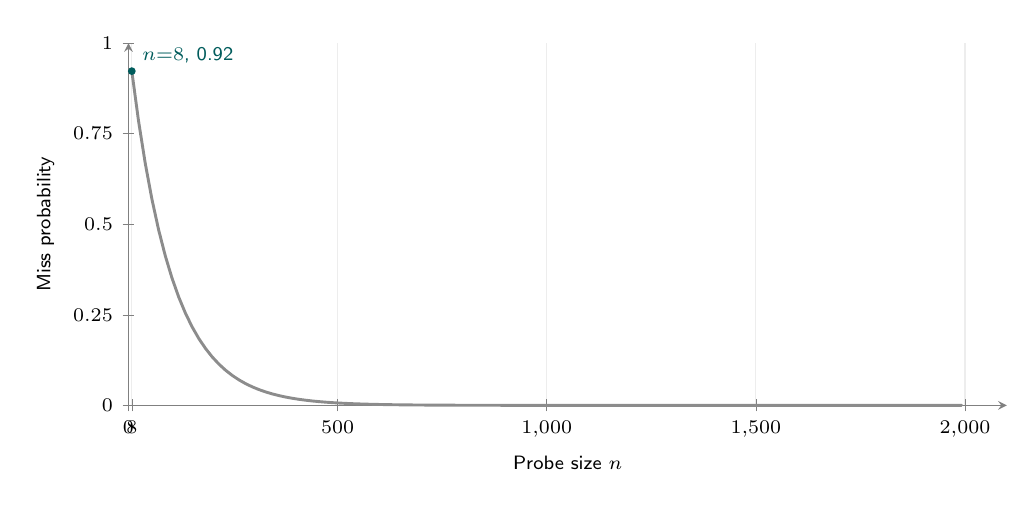
\begin{tikzpicture}
\begin{axis}[
  acts,
  width=0.92\columnwidth,
  height=4.6cm,
  xmin=0, xmax=2100,
  ymin=0, ymax=1,
  xlabel={Probe size $n$},
  ylabel={Miss probability},
  xtick={0,8,500,1000,1500,2000},
  ytick={0,0.25,0.5,0.75,1},
]
% source: PROJECTED (1-0.01)^n, drawn at every 16 from 8 to 2000
\addplot[actsghost, line width=1.05pt, mark=none] coordinates {(8,0.92274469) (24,0.78567814) (40,0.66897176) (56,0.5696012) (72,0.48499137) (88,0.41294967) (104,0.35160921) (120,0.29938039) (136,0.25490976) (152,0.2170449) (168,0.18480456) (184,0.15735328) (200,0.13397967) (216,0.11407804) (232,0.09713263) (248,0.082704332) (264,0.070419247) (280,0.059959015) (296,0.051052569) (312,0.043469107) (328,0.037012109) (344,0.031514248) (360,0.026833051) (376,0.02284721) (392,0.019453434) (408,0.016563778) (424,0.014103357) (440,0.012008413) (456,0.010224657) (472,0.0087058634) (488,0.0074126751) (504,0.0063115798) (520,0.0053740437) (536,0.0045757712) (552,0.003896076) (568,0.0033173442) (584,0.0028245785) (600,0.0024050093) (616,0.0020477639) (632,0.0017435844) (648,0.0014845885) (664,0.0012640644) (680,0.0010762975) (696,0.00091642186) (712,0.00078029451) (728,0.00066438783) (744,0.00056569818) (760,0.00048166811) (776,0.00041012006) (792,0.00034919991) (808,0.00029732898) (824,0.00025316307) (840,0.00021555766) (856,0.00018353825) (872,0.00015627507) (888,0.00013306162) (904,0.00011329635) (920,9.6467057e-05) (936,8.2137625e-05) (952,6.9936719e-05) (968,5.9548163e-05) (984,5.0702746e-05) (1000,4.3171247e-05) (1016,3.6758494e-05) (1032,3.1298305e-05) (1048,2.6649185e-05) (1064,2.2690656e-05) (1080,1.9320135e-05) (1096,1.6450279e-05) (1112,1.4006718e-05) (1128,1.1926129e-05) (1144,1.0154595e-05) (1160,8.6462091e-06) (1176,7.3618819e-06) (1192,6.2683316e-06) (1208,5.3372196e-06) (1224,4.5444171e-06) (1240,3.8693793e-06) (1256,3.2946131e-06) (1272,2.8052239e-06) (1288,2.3885297e-06) (1304,2.0337322e-06) (1320,1.731637e-06) (1336,1.4744158e-06) (1352,1.2554028e-06) (1368,1.0689225e-06) (1384,9.1014235e-07) (1400,7.7494778e-07) (1416,6.5983531e-07) (1432,5.618219e-07) (1448,4.7836762e-07) (1464,4.0730983e-07) (1480,3.4680712e-07) (1496,2.9529162e-07) (1512,2.5142834e-07) (1528,2.1408062e-07) (1544,1.822806e-07) (1560,1.5520424e-07) (1576,1.3214985e-07) (1592,1.1252002e-07) (1608,9.5806045e-08) (1624,8.1574802e-08) (1640,6.9457499e-08) (1656,5.9140127e-08) (1672,5.0355321e-08) (1688,4.2875429e-08) (1704,3.6506617e-08) (1720,3.1083843e-08) (1736,2.646658e-08) (1752,2.2535175e-08) (1768,1.918775e-08) (1784,1.6337559e-08) (1800,1.3910741e-08) (1816,1.1844409e-08) (1832,1.0085014e-08) (1848,8.5869635e-09) (1864,7.3114368e-09) (1880,6.2253797e-09) (1896,5.3006479e-09) (1912,4.5132778e-09) (1928,3.8428655e-09) (1944,3.2720377e-09) (1960,2.7860019e-09) (1976,2.372163e-09) (1992,2.0197966e-09)};
\fill[actsteal] (axis cs:8,0.92274469) circle[radius=1.4pt];
\node[actlab, anchor=south west, text=actsteal, xshift=2pt, yshift=1pt] at (axis cs:8,0.92274469) {$n{=}8$, 0.92};
\end{axis}
\end{tikzpicture}
